\documentclass[12pt, oneside]{book}
\usepackage[a4paper,top=2.5cm,bottom=2.5cm,left=3.5cm,right=2cm]{geometry}
\usepackage[utf8]{inputenc}
\usepackage[T1]{fontenc}  
\usepackage{graphicx}
\usepackage{url}
\usepackage{listings}
\usepackage[slovak]{babel} % vypnite pre prace v anglictine
\linespread{1.25} % hodnota 1.25 by mala zodpovedat 1.5 riadkovaniu
\usepackage{tabularx}
\usepackage{fancyhdr}
\usepackage{float}
\usepackage{color}





\definecolor{codegreen}{rgb}{0,0.6,0}
\definecolor{codegray}{rgb}{0.5,0.5,0.5}
\definecolor{codepurple}{rgb}{0.58,0,0.82}
\definecolor{backcolour}{rgb}{1,1,1}

\lstdefinestyle{mystyle}{
	backgroundcolor=\color{backcolour},   
	commentstyle=\color{codegreen},
	keywordstyle=\color{magenta},
	numberstyle=\tiny\color{codegray},
	stringstyle=\color{codepurple},
	basicstyle=\footnotesize,
	breakatwhitespace=false,         
	breaklines=true,                 
	captionpos=b,                    
	keepspaces=true,                 
	numbers=none,                    
	numbersep=5pt,                  
	showspaces=false,                
	showstringspaces=false,
	showtabs=false, 
	inputencoding=utf8,
	extendedchars=true,
literate=
{á}{{\'a}}1 {é}{{\'e}}1 {í}{{\'i}}1 {ó}{{\'o}}1 {ú}{{\'u}}1
{č}{{\'c}}1 {ť}{{\'t}}1 {ž}{{\'z}}1
{Á}{{\'A}}1 {É}{{\'E}}1 {Í}{{\'I}}1 {Ó}{{\'O}}1 {Ú}{{\'U}}1
{à}{{\`a}}1 {è}{{\`e}}1 {ì}{{\`i}}1 {ò}{{\`o}}1 {ù}{{\`u}}1
{À}{{\`A}}1 {È}{{\'E}}1 {Ì}{{\`I}}1 {Ò}{{\`O}}1 {Ù}{{\`U}}1
{ä}{{\"a}}1 {ë}{{\"e}}1 {ï}{{\"i}}1 {ö}{{\"o}}1 {ü}{{\"u}}1
{Ä}{{\"A}}1 {Ë}{{\"E}}1 {Ï}{{\"I}}1 {Ö}{{\"O}}1 {Ü}{{\"U}}1
{â}{{\^a}}1 {ê}{{\^e}}1 {î}{{\^i}}1 {ô}{{\^o}}1 {û}{{\^u}}1
{Â}{{\^A}}1 {Ê}{{\^E}}1 {Î}{{\^I}}1 {Ô}{{\^O}}1 {Û}{{\^U}}1
{œ}{{\oe}}1 {Œ}{{\OE}}1 {æ}{{\ae}}1 {Æ}{{\AE}}1 {ß}{{\ss}}1
{ű}{{\H{u}}}1 {Ű}{{\H{U}}}1 {ő}{{\H{o}}}1 {Ő}{{\H{O}}}1
{ç}{{\c c}}1 {Ç}{{\c C}}1 {ø}{{\o}}1 {å}{{\r a}}1 {Å}{{\r A}}1
{€}{{\EUR}}1 {£}{{\pounds}}1,                 
	tabsize=2
}

\lstset{style=mystyle}


% -------------------
% --- Definicia zakladnych pojmov
% --- Vyplnte podla vasho zadania
% -------------------
\def\mfrok{2016}
\def\mfnazov{Workflow management rolí a užívateľov}
\def\mftyp{Bakalárska práca}
\def\mfautor{Pavol Martiš}
\def\mfskolitel{prof. RNDr. Gabriel Juhás, PhD.}
\def\mfevidenceneCislo{FEI-5382-72557}

%ak mate konzultanta, odkomentujte aj jeho meno na titulnom liste
\def\mfkonzultant{tit. Meno Priezvisko, tit. }  

\def\mfmiesto{Bratislava, \mfrok}

%aj cislo odboru je povinne a je podla studijneho odboru autora prace
\def\mfodbor{ 9.2.9 aplikovaná informatika } 
\def\program{ Aplikovaná informatika }
\def\mfpracovisko{ Ústav informatiky a matematiky }



%moje funkcie 
\newcommand{\mychapter}[2]{
	\stepcounter{chapter}
	\setcounter{chapter}{#1}
	\setcounter{section}{0}
	\chapter*{#2}
	\markboth{chapter name}{}
	\addcontentsline{toc}{chapter}{#2}
}

\newcounter{listOfAppendix}


\def\@zoznamPri{Pr\'{i}lohy}








\begin{document}     

% -------------------
% --- Obalka ------
% -------------------
\thispagestyle{empty}

\begin{center}
\sc\large
Slovenská technická univerzita
\\*Fakulta elektrotechniky a informatiky\\
\end{center}


{	
	Evidenčné číslo: \mfevidenceneCislo
	\noindent 
}

\vfill
\begin{center}
{\LARGE\mfnazov}\\
\Large\mftyp
\end{center}

\vfill

{\sc\large 
\noindent \mfrok\\
\mfautor
}

\eject % EOP i
% --- koniec obalky ----

% -------------------
% --- Titulný list
% -------------------

\thispagestyle{empty}
\noindent

\begin{center}
\sc  
\large
Slovenská technická univerzita v Bratislave\\
Fakulta elektrotechniky a informatiky\\
\end{center}
\begin{tabular}{ll}
Evidenčné číslo: \mfevidenceneCislo
\end{tabular}

\vfill

\begin{center}
{\LARGE\mfnazov}\\
\Large \mftyp
\end{center}

\vfill

\noindent
\begin{tabular}{ll}
Študijný program: & \program \\
Študijný odbor: & \mfodbor \\
Školiace pracovisko: & \mfpracovisko \\
Školiteľ: & \mfskolitel \\
% Konzultant: & \mfkonzultant \\
\end{tabular}

\vfill


\noindent \mfmiesto\\
\mfautor

\eject % EOP i


% --- Koniec titulnej strany


% -------------------
% --- Zadanie z AIS
% -------------------
% v tlačenej verzii s podpismi zainteresovaných osôb.
% v elektronickej verzii sa zverejňuje zadanie bez podpisov

\newpage 
\thispagestyle{empty}
\hspace{-2cm}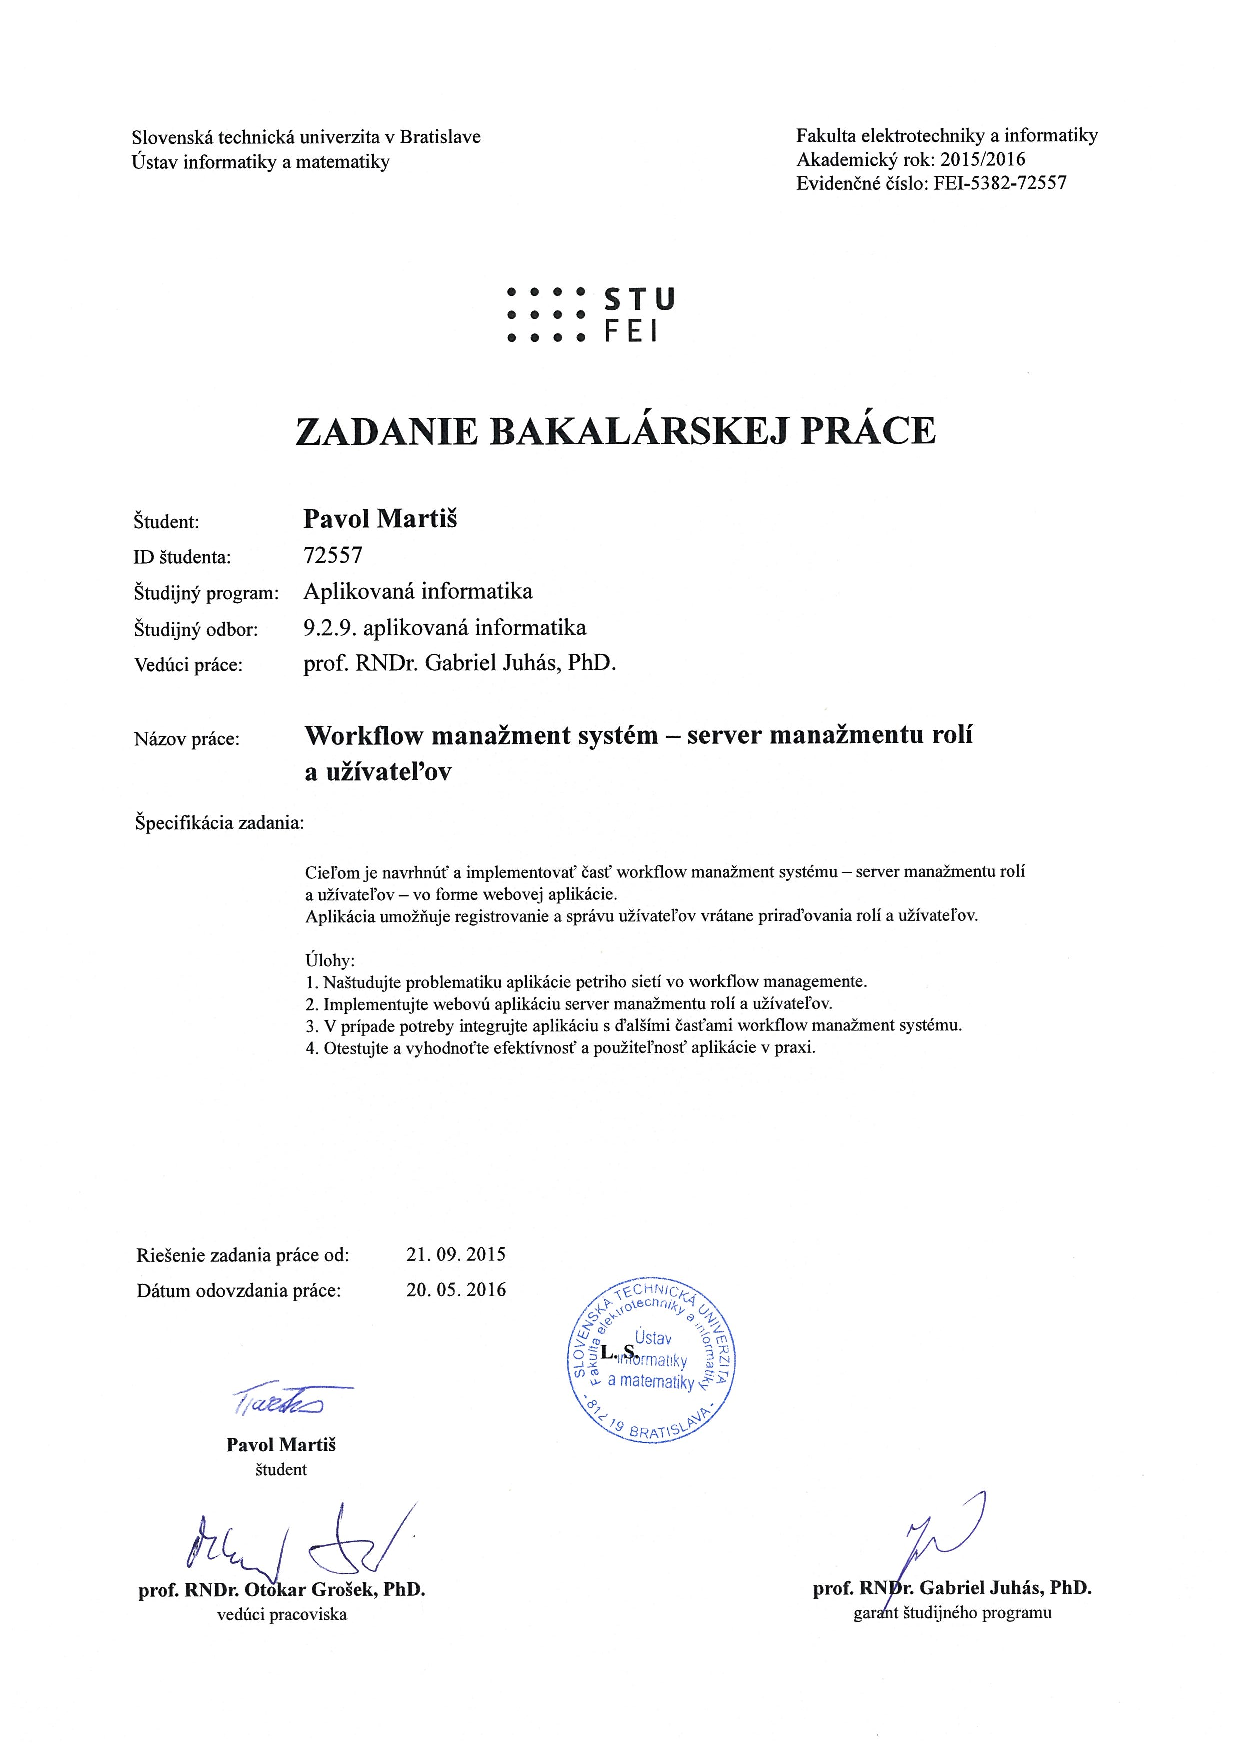
\includegraphics[width=1.1\textwidth]{images/zadanie}

% --- Koniec zadania

\frontmatter


%---------------
% Čestné vyhlásenie
% ----------------
\setcounter{page}{3}
\newpage 
\noindent
\vfill
\begin{center}
	\LARGE \textbf{Vyhlásenie autora}  \\
\end{center}
Podpísaný Pavol Martiš čestne vyhlasujem, že som Bakalársku prácu Workflow manažment systém – server manažmentu rolí a užívateľov vypracoval na základe poznatkov získaných počas štúdia a informácií z dostupnej literatúry uvedenej v práci.\\
Uvedenú prácu som vypracoval pod vedením Prof. RNDr. Gabriela Juhása, PhD.
V Bratislave dňa 15.05.2016 \\\\\\



..................................................\\\\
\indent podpis autora

\vfill

% -------------------
%   Poďakovanie - nepovinné
% -------------------
\setcounter{page}{4}
\newpage 
\begin{center}
	\LARGE \textbf{Poďakovanie}  \\
\end{center}
\indent Chcel by som poďakovať všetkým, ktorí mi akýmkoľvek spôsobom pomohli pri spracovaní
tejto bakalárskej práce. Moje poďakovanie patrí najmä vedúcemu práce, prof. RNDr. Gabrielovi Juhásovi, PhD., za
vedenie a celému tímu študentov, ktorí sa spoločne podieľali na tvorbe Workflow manažment systému.

\noindent Osobitné poďakovanie patrí mojej rodine, ktorá ma psychicky podporovala.
\noindent  

\vfill


% --- Koniec poďakovania

% -------------------
%   Abstrakt - Slovensky
% -------------------
%\newpage 
%\section*{Abstrakt}


%Slovenský abstrakt v rozsahu 100-500 slov, jeden odstavec. Abstrakt
%stručne sumarizuje výsledky práce. Mal by byť pochopiteľný pre bežného
%informatika. Nemal by teda využívať skratky, termíny alebo označenie
%zavedené v práci, okrem tých, ktoré sú všeobecne známe.

%\%paragraph*{Kľúčové slová:} užívateľ, rola , workflow, Petriho sieť, RBAC , workflow
% --- Koniec Abstrakt - Slovensky


\newpage
\pagestyle{empty}	
\section*{\fontsize{22pt}{1.3}\selectfont S\'{U}HRN}
\noindent SLOVENSKÁ TECHNICKÁ UNIVERZITA V BRATISLAVE
\newline
FAKULTA ELEKTROTECHNIKY A INFORMATIKY \\
\begin{tabbing}	
	\hspace*{7cm}\= \kill
	\v{S}tudijný 	program:\> Aplikovaná informatika\\
	Autor:\> \mfautor\\
	Bakalárska práca  :\>
	\begin{minipage}[t]{20em}
		Bakalárska práca: Workflow manažment systém - server manažmentu rolí a užívateľov
	\end{minipage} \\
	Vedúci záverečnej práce :\> prof. RNDr. Gabriel Juhás, PhD.\\
	
	Miesto a rok predlo\v{z}enia pr\a'ace :\>Bratislava 2016
\end{tabbing}
Práca sa zaoberá návrhom serveru rolí pre Workflow manažment systém. Je rozdelená do troch častí. V prvej časti analyzuje problematiku Petriho sietí , Workflow manažmentu a metód riadenia prístupu. V druhej sa zaoberá architektúrou Workflow systému a bližšie rozoberá ich jednotlivé časti.
\\ \\
\paragraph*{Kľúčové slová:} 
 Workflow manažment systém, Petriho siete, server manažmentu rolí, rola

% -------------------
% --- Abstrakt - Anglicky 
% -------------------
\newpage
\pagestyle{empty}	
\section*{\fontsize{21pt}{1.3}\selectfont ABSTRACT}
 
	\noindent SLOVAK UNIVERSITY OF TECHNOLOGY IN BRATISLAVA
	\newline
	{\fontsize{11pt}{1.3}\selectfont FACULTY OF ELECTRICAL ENGINEERING AND INFORMATION TECHNOLOGY\\ }
	


\begin{tabbing}	
	\hspace*{7cm}\= \kill
	Study Programme :\> Applied Informatics\\
	Author :\> \mfautor\\
	Bachelor Thesis :\>
	\begin{minipage}[t]{20em}
	Workflow management system - server of role management
	and organizational structure
	\end{minipage} \\
	Supervisor :\> prof. RNDr. Gabriel Juhás, PhD.\\
	
	Place and year of submission :\>Bratislava 2016
\end{tabbing}
gfdsgdfs
\\ \\


\paragraph*{Keywords:} 

% --- Koniec Abstrakt - Anglicky

% -------------------
% --- Predhovor - v informatike sa zvacsa nepouziva
% -------------------
%\newpage 
%\thispagestyle{empty}
%
%\huge{Predhovor}
%\normalsize
%\newline
%Predhovor je všeobecná informácia o práci, obsahuje hlavnú charakteristiku práce 
%a okolnosti jej vzniku. Autor zdôvodní výber témy, stručne informuje o cieľoch 
%a význame práce, spomenie domáci a zahraničný kontext, komu je práca určená, 
%použité metódy, stav poznania; autor stručne charakterizuje svoj prístup a svoje 
%hľadisko. 
%
% --- Koniec Predhovor


% -------------------
% --- Obsah
% -------------------

\newpage 


\tableofcontents



% ---  Koniec Obsahu

% -------------------
% --- Zoznamy tabuliek, obrázkov - nepovinne
% -------------------

\newpage 

{\LARGE Zoznam skratiek}\\

\noindent
WFMS – Workflow management system\\
RBAC – Role-based access control\\
MVC - Model-view-controller\\
DAC - Discretionary Access Control\\
MAC - Mandatory access control\\
ACL - Access control list\\
NIST - National Institute of Standards and Technology\\
MLS - Multilevel security\\
SVG - Scalable Vector Graphics\\
XML - Extensible Markup Language\\
JSON - JavaScript Object Notation\\
CSS - Cascading Style Sheets\\
PHP - 
MySQL - 

\listoffigures



% ---  Koniec Zoznamov

\mainmatter


\input uvod.tex 

\input analyza.tex

\input opis.tex

\input opisroli.tex

\input zaver.tex

% -------------------
% --- Bibliografia
% -------------------


\newpage

\backmatter

\thispagestyle{empty}
\nocite{*}
\clearpage

%\bibliographystyle{plain}

%\bibliography{literatura} 

%Prípadne môžete napísať literatúru priamo tu
\begin{thebibliography}{5}
 
\bibitem{gabova_kniha} MOLINA H. G. - ULLMAN J. D. - WIDOM J., 2002, Database Systems, Upper Saddle River : Prentice-Hall, 2002, 1119 s., Pearson International edition, 0-13-098043-9

\bibitem{workflow_systemy}
AALST, W.: \textit{The Application of Petri Nets to Workflow Management}. Dostupné
na internete: http://wwwis.win.tue.nl/ wvdaalst/publications/p53.pdf

\bibitem{autorizacia}
Shengli Wu - Amit Sheth - John Miller - Zongwei Luo:\textit{ Authorisation and Access Control of Application Data
	in Workflow Systems}: Journal of Intelligent Information Systems, 2002, č.18, s.71-94

\bibitem{ekonomika}Michael P. Gallaher - Alan C. O'Connor - Brian Kropp, \textit{ The Economic Impact
of Role-Based Access Control}, National Institute of Standards and Technology,
2002.Dostupné na internete: http://www.nist.gov/director/planning/upload/report02-1.pdf

\bibitem{kuhn}D. Ferraiolo - D.R. Kuhn - R. Chandramouli: \textit{Role-based Access Control}. Artech
House Computing Library. Artech House, 2007, 405 s., ISBN 9781596931138


\bibitem{aalst}AALST, W. - HEE, K.: \textit{Workflow Management Models, methods and systems}. Cambridge,
Massachusetts: The MIT Press, 2004, ISBN 0-262-01189-1, p.
267-268

\bibitem{workflow_vyhody}W. M. Van Der Aalst: \textit{Three good reasons for using a petri-net-based workflow
management system}. Medzinárodná vedecká konferencia o informáciach a integrácii procesov v podnikoch (IPIC’96)
s. 179–201 , 1996.

\bibitem{saltzer}J. H. Saltzer - M. D. Schroeder: \textit{The Protection of Information in Computer
Systems}.  IEEE, č.63, September 1975, s.1278–1308.

\bibitem{belapadula}
D. E. Bell - L. J. La Padula: Secure computer systems: Vol. I—mathematical
foundations,  Vol. II—a mathematical model,  Vol. III—a refinement of the mathematical
model. Technical Report MTR-2547 (tri zväzky). Bedford: Mitre Corporation, MA, 1973.

\bibitem{sandhu96}Sandhu, R. a kol.: \textit{Role-Based Access Control Models}. IEEE Computer, zväzok.
29, č. 2, 1996.

\bibitem{NIST95}Ferraiolo, D. F. -  J. Cugini, - D. R. Kuhn:\textit{ Role-Based Access Control
(RBAC): Features and Motivations}.  New Orleans, LA : Konferencia o bezpečnosti aplikácii
, December 11–15, 1995,
s. 241–248.

\bibitem{telecom}Telecom Glossary 2000, American National Standard for Telecommunications, American National Standards Institute

\bibitem{TSCES}DoD, Trusted Computer System Evaluation Criteria (TCSEC), DoD 5200.28-STD.

\bibitem{MAC}CURPHEY, Mark:\textit{ Mandatory Access Control} [online]. 2002 [cit. 2008-10-22] .
 Dostupné na internete: <http://www.cgisecurity.com/owasp/html/ch08s02.html>

\bibitem{Modelovacie_formalizmy}JUHÁS, G.: \textit{Modelovacie formalizmy udalostných systémov}. Bratislava: RT systems
s.r.o., 2011, ISBN 978-80-970519-1-4, p. 29-45	

\bibitem{desel}DESEL, J. - REISIG, W.: Lectures on Petri nets I: Basic models. Germany: Universtit
ät Karlsruhe: Springer, 1998, ISBN 3-540-65306-6

\bibitem{petri}PETRI, C.A. - REISIG, W. 2008 Petri net. [online] [cit. 27.04.2016]. Dostupné na internete:
 <http://www.scholarpedia.org/article/Petri\_net>
 
 \bibitem{page_speed}PageSpeed Insights [online] . Dostupné na internete:  <https//developers.google.com/speed/pagespeed/>
 
  \bibitem{attensee}Attensee [online] . Dostupné na internete> <http://www.attensee.com/ >



\end{thebibliography}

%---koniec Referencii

% -------------------
%--- Prilohy---
% -------------------

%Nepovinná časť prílohy obsahuje materiály, ktoré neboli zaradené priamo  do textu. Každá príloha sa začína na novej strane.
%Zoznam príloh je súčasťou obsahu.
%
%\addcontentsline{toc}{chapter}{Appendix A}
%\input AppendixA.tex
%
%\addcontentsline{toc}{chapter}{Appendix B}
%\input AppendixB.tex

\newpage
\renewcommand \thesection{\Alph{section}}
\setcounter{section}{0}
\setcounter{subsection}{0}
\setcounter{subsubsection}{0}
\renewcommand \thetable{\Alph{section}}
\setcounter{table}{0}
\setcounter{figure}{0}
\setcounter{page}{1}  
\pagenumbering{Roman}
\cleardoublepage
\addcontentsline{toc}{section}{\@zoznamPri}

\section{Štruktúra elektronického nosiča}

\end{document}






